\section*{Question 1:}
Exercise 6.2: 

Create a simple spelling corrector based on the noisy channel model. Use a single-word language model, and an error model where all errors with the same edit distance have the same probability. Only consider edit distances of 1 or 2. Implement your own edit distance calculator (example code can easily be found on the Web).

\subsection*{Answer:}

\textbf{Summary of the noisy channel model approach:}

Let $M$ be the misspelled word we want to correct.

Let $W$ be the array of possible corrections to $M$ where $W = \{w_i | i = 1, 2, 3, ..., n\}$.

Computing conditional probability $CP$ for each possible correct word, element in $W$, gives us: $CP_i = P(M|w_i) \times P(w_i)$ for $i = 1, 2, 3, ..., n$

Choose $w_i$ that maximizes $CP_i$

\textbf{Implementation:}

I found an example code on the web and modified it as the question suggested. The program file is named ``correct.py''. It takes one command line argument, the word we are trying to correct, and it prints out the correct spelling and exits. The program, by design, will have to be launched again to correct another word. 

\lstinputlisting[language=Python, breakatwhitespace=〈false), label=The content of correct.py, caption= The content of correct.py]{Q1/correct.py}

\begin{figure}[h]
\caption{Running correct.py}
\centering
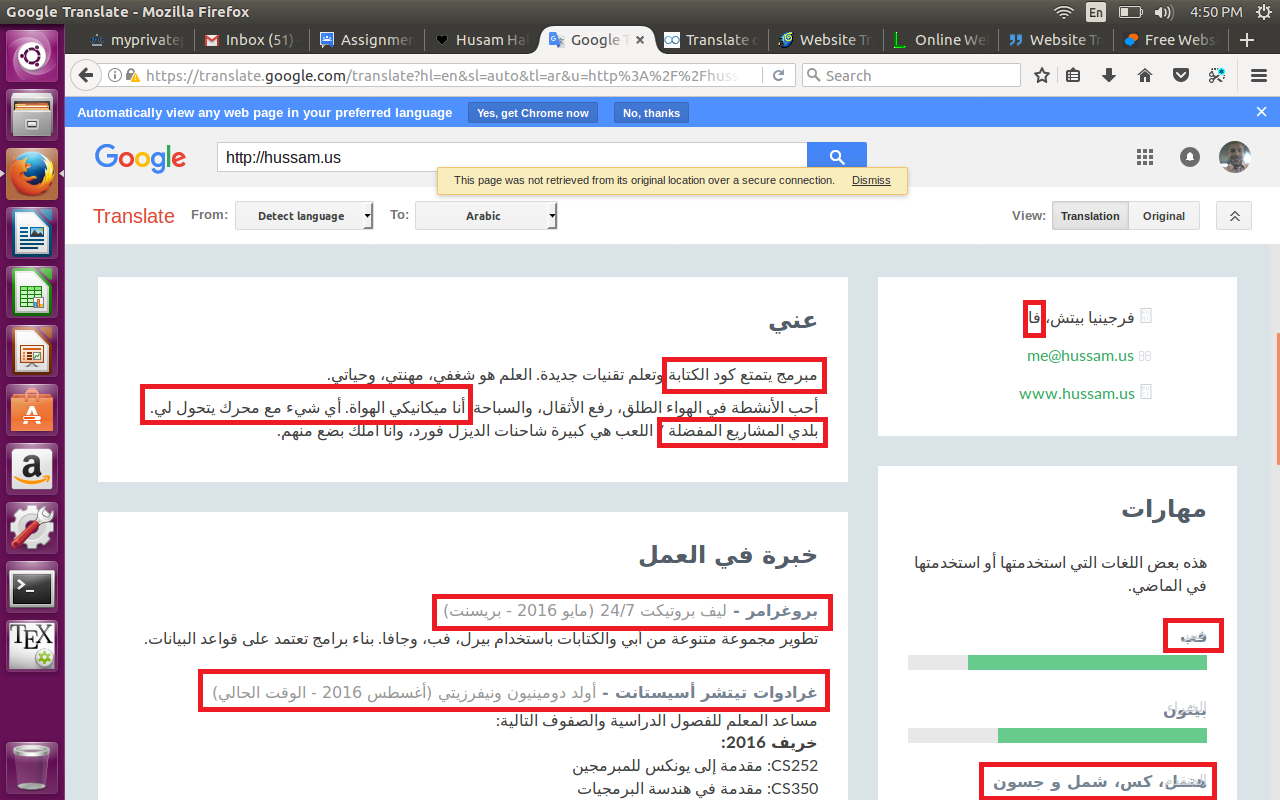
\includegraphics[scale=0.8]{Q1/1.png}
\end{figure}



